%%%%%%%%%%%%%%%%%%%%%%%%%%%%%%%%%%%%%%%%%
% CN2 Labreport template
%
% License:
% CC BY-NC-SA 3.0 (http://creativecommons.org/licenses/by-nc-sa/3.0/)
%
%%%%%%%%%%%%%%%%%%%%%%%%%%%%%%%%%%%%%%%%%

\documentclass[parskip=full]{scrartcl}

\usepackage{siunitx}  % Provides the \SI{}{} command for typesetting SI units
\usepackage{graphicx} % Required for the inclusion of images
\usepackage{booktabs} % nicer tables
\usepackage[noabbrev]{cleveref} % automatic references
\usepackage{listings} % typeset code
\usepackage[backend=biber]{biblatex}
\addbibresource{referenzen.bib}

\crefname{lstlisting}{listing}{listings} % for referencing code
\Crefname{lstlisting}{Listing}{Listings} % for referencing code

\usepackage[headsepline]{scrlayer-scrpage} % header
\ohead{Group 06} % right part of header
\ihead{Assignment 1} % left part of header

\lstset{basicstyle=\ttfamily} % monospaced font in listing



%----------------------------------------------------------------------------------------
%	DOCUMENT INFORMATION
%----------------------------------------------------------------------------------------

\begin{document}
\begin{titlepage}
    \centering
    \vspace*{2cm}
    {\Huge \textbf{Communication Networks 2}}\\
    SS 2021\\
    \vspace*{1cm}
    {\Large Assignment 2}
    \\\vspace*{3cm}
    {\Large \textbf{Group 06}}\\
    \vspace*{1cm}
    {\large 
        \begin{tabular}{l c c}
            Name & Mat.Nummer \\ \hline
            Paul Kloker & 12034928 \\
            Juan Aramis Oposich & 11701238
        \end{tabular}
    }
    \\\vspace*{7cm}
    \today
\end{titlepage}

%----------------------------------------------------------------------------------------
%	SECTION 1
%----------------------------------------------------------------------------------------
\section{Task description} \label{sec:task}
The task of this assignment is to set up a Voice over IP (VoIP) Client and compare the influence of multimedia codecs on the Quality of Service (QoS) of video calls.
Furthermore, the signaling messages of the Session Initiation Protocol (SIP) shall be analyzed to verify the correct behavior and to find a secret message of the registrar.

The comparison of the QoS is to be done once subjectively and once on the basis of self-selected network parameters, which are also to be visualized graphically. 


%----------------------------------------------------------------------------------------
%	SECTION 2
%----------------------------------------------------------------------------------------
\section{Procedure} \label{sec:procedure}

\subsection{Linphone setup and SIP registration} \label{subsec:setup}
Before a VoIP call can be done, one of the first thing is to do a SIP registration. SIP Endpoints are identified by their Address of Record, for example "sip:cn\_06@cn2lab.cn.tuwien.at".

The endpoint is also defined by the location, which is identified by an IP address, port number and protocol. To receive calls, the caller needs to know the location of the callee. Since most SIP endpoints do not have a permanent, fixed, publicly-reachable IP address, they will need to register with a central server, or Registrar, so that they can receive incoming calls. This server accepts REGISTER requests and places the information it receives in those requests into the location service for the domain it handles. In figure \labelcref{fig:SIP Registrar}

\begin{figure}[!ht]
	\centering % centering figure 
	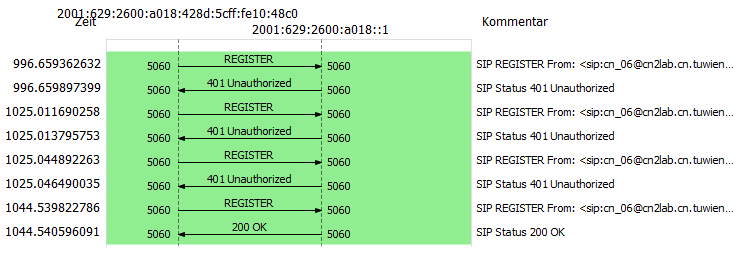
\includegraphics[height=6cm]{images/sip_flowseq.png} % importing figure
	\caption{SIP registration flow} 
	\label{fig:SIP Registrar} % labeling to refer it inside the text
\end{figure} 

The first sequence is the initial registration request from SIP User Agent with it's address information. The SIP registrar answers with the information about the login "401 Unauthorized". To be authenticate, the client will combine a received nonce with his user and password information and create an MD5 hash out of them. A successful login is omitted with a 200 OK.

\subsubsection{secret message}
One of the task was to extract a secret message from the registration process. The secret message can be found in the last step of the registrar.

\begin{itemize}
	\item SIP REQUEST: Digest realm="cn2lab.cn.tuwien.ac.at", nonce="YJpM2mCaS64RWAT+53QLYY40A29xCJ3l", username="cn\_06",  uri="sip:cn2lab.cn.tuwien.ac.at", response="aa76de94237e27cb05b0091b89a01628"
	\item STATUS 200 OK: Secret-Message: Dazecixaru4
\end{itemize}

\subsection{Capturing process} \label{subsec:capture}
This year because of the COVID-19 pandemic it was only possible to access the lab PCs remotely.
This is most of the time no problem but to compare the video and audio quality of SIP calls it is important to have direct access, because the VNC connection influences the subjective impressions.
To overcome this problem a command line tool called \verb|cn2_sbs_capture| has been provided, which captures the incoming audio and video and the outgoing video.
Because the camera and microphone of the lab PC could not be used the same video was played each call.

To capture a call, the selected codecs were first set in the Linphone settings. 
Then \verb|cn2_sbs_capture| was executed with the default settings and the Wireshark capture was started. 
After that a one-minute-long call was made. 
Table \ref{tab:capture} shows all captured calls and the chosen codecs.

\begin{table}[hb]
	\centering
	\caption{Captured calls}
	\label{tab:capture}
	\begin{tabular}{l|l|l|l}
		\toprule
		\textbf{No.} & \textbf{connection type} & \textbf{video codec} & \textbf{audio codec}  \\ \midrule
		1 & landline & VP8 & OPUS\\
		2 & satellite & VP8 & OPUS\\
		3 & landline & MP4V\_ES & speex 16 kbit\\
		4 & satellite & MP4V\_ES & speex16 kbit\\
		5 & landline & MP4V\_ES & PCMU\\
		6 & satellite & MP4V\_ES & PCMU\\
		7 & satellite & H.263-1998\_ES & GSM\\
		8 & satellite & H.263 & speex 8 kbit\\
		\bottomrule
	\end{tabular}
\end{table}

- Wie sind wir vorgegangen um alle unterschiedlichen Codecs zu capturen... (+cn2\_sbs\_capture  tool)
\subsection{SIP signaling and SDP} \label{subsec:signaling}

- SIP Signaling mit Sequenzdiagramm beschreiben "verify that both, signaling and media work correctly."

- SDP genauer anschauen (stehen die ausgewählten codecs drinnen...)
\subsection{Audio codec quality comparison} \label{subsec:audio}
- Audio codecs subjektiv  vergleichen (vielleicht nach der Mean Opinion Score)

- RTP Analyse + Grafen
\subsection{Video codec quality comparison} \label{subsec:video}
- Video codecs subjektiv vergleichen  

z.B.\verb| https://en.wikipedia.org/wiki/Subjective_video_quality | 
  
Das ist so ähnlich wie MOS:
https://www.irisa.fr/armor/lesmembres/Mohamed/Thesis/node146.html

- RTP Analyse + Grafen
%----------------------------------------------------------------------------------------
%	SECTION 3
%----------------------------------------------------------------------------------------
\section{Conclusion}

Was sind die besten Codecs für welche Situation. 
%----------------------------------------------------------------------------------------
%	SECTION X
%---------------------------------------------------------------------------------------

\printbibliography

\end{document}
